\section{Problem (6)}
	Three connected blocks are pulled to the right on a horizontal frictionless table by a force of magnitude $T_{3} = 58 \ N$. If $m_{1} = 13 \ kg$, $m_{2} = 26 \ kg$, and $m_{3} = 34 \ kg$.

	\begin{figure}[H]
		\begin{center}
			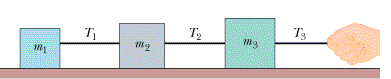
\includegraphics[scale=1]{hw5_problem6}
			\caption{Illustration of Problem 6}
			\label{fig:hw5_problem6}
		\end{center}
	\end{figure}

	\subsection{Question (a)}

		Calculate the magnitude of the system's acceleration:

		\textbf{R:} \newline

		\begin{figure}[H]
			\begin{center}
				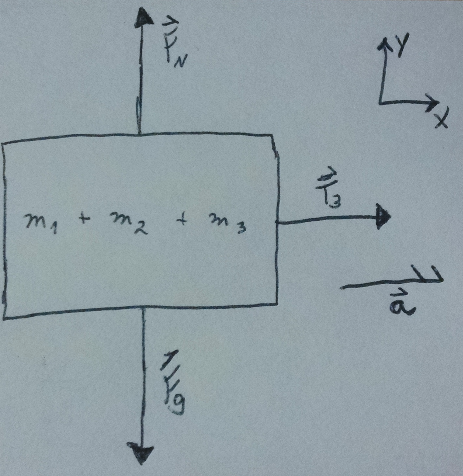
\includegraphics[scale=0.5]{hw5_problem6a_fbd}
				\caption{Free-Body Diagram (Problem 6 (a))}
				\label{fig:hw5_problem6a_fbd}
			\end{center}
		\end{figure}

		\begin{align}
			m = \ &m_{1} + m_{2} + m_{3}& \notag \\
			= \ &73 \ kg& \notag
		\end{align}

		Newton's $2^{nd}$ Law on Block $3$:
		\begin{align}
			\sum F_{x} = \ &ma_{x}& \notag \\
			T_{3} = \ &(73 \ kg)a_{x}& \notag \\
			a_{x} = \ &\frac{58 \ N}{73 \ kg}& \notag \\
			a = \ &0.8 \ m/s^{2}&
		\end{align}

	\subsection{Question (b)}

		Calculate the tension $T_{1}$:

		\textbf{R:} \newline

		\begin{figure}[H]
			\begin{center}
				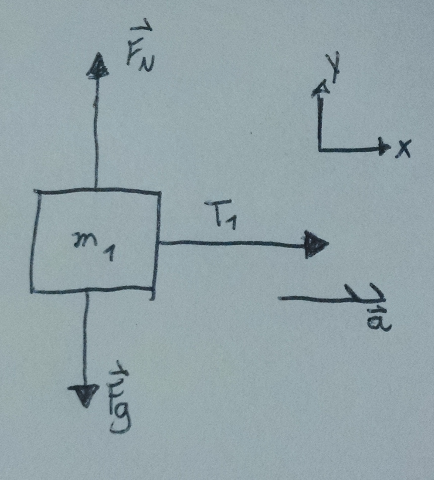
\includegraphics[scale=0.7]{hw5_problem6b_fbd}
				\caption{Free-Body Diagram (Problem 6 (b))}
				\label{fig:hw5_problem6b_fbd}
			\end{center}
		\end{figure}

		Newton's $2^{nd}$ Law on Block $1$:
		\begin{align}
			\sum F_{x} = \ &ma_{x}& \notag \\
			T_{1} = \ &(13 \ kg)(0.8 \ m/s^{2})& \notag \\
			= \ &10.4 \ N&
		\end{align}

	\subsection{Question (c)}

		Calculate the tension $T_{2}$:

		\textbf{R:} \newline

		\begin{figure}[H]
			\begin{center}
				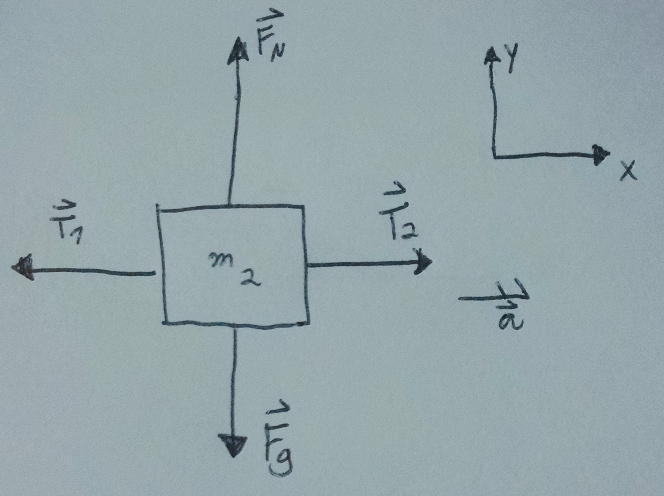
\includegraphics[scale=0.5]{hw5_problem6c_fbd}
				\caption{Free-Body Diagram (Problem 6 (c))}
				\label{fig:hw5_problem6c_fbd}
			\end{center}
		\end{figure}

		Newton's $2^{nd}$ Law on Block $2$:
		\begin{align}
			\sum F_{x} = \ &ma_{x}& \notag \\
			T_{2} - T_{1} = \ &(26 \ kg)(0.8 \ m/s^{2})& \notag \\
			T_{2} = \ &(20.8 \ N) + (10.4 \ N)& \notag \\
			= \ &31.2 \ N&
		\end{align}
